\documentclass[11pt,a4paper,oneside, openright]{article}
\usepackage[left=3cm,right=3cm, top=3cm, bottom=3cm]{geometry}
\usepackage{graphicx}
\usepackage[british]{babel}
\usepackage[utf8]{inputenc}
\usepackage{mathtools}
\usepackage{setspace}
\usepackage{verbatim}
\usepackage[htt]{hyphenat}
\usepackage{url}
\usepackage{amsmath}
\usepackage{placeins}
\usepackage{caption}
\usepackage{subcaption}
\usepackage[bookmarks]{hyperref}


\begin{document}
{\setstretch{1.0}
  \begin{titlepage}
  	\centering
  	
\includegraphics[width=6cm]{images/unipi.eps}\par
  	\vspace{1.5cm}
  	{\huge\textsc{Performance evaluation of a CRAN system}\par}
  	\vspace{2cm}
  	Gerardo \textsc{Alvaro}\par
  	Francesco \textsc{Barbarulo}\par
    Francesco \textsc{Fornaini}

  	\vfill

    % Bottom of the page
  	{\large 2018-2019\par}
  \end{titlepage}
}


\tableofcontents

\newpage

\section{Introduction}
\label{sec:introduction}

The system examined is a simplified version of an architecture presented for future cellular networks, called Cloud-RAN (CRAN).

\subsection{Description of the system}
 At the center of this system there is a central processing unit (BBU), which is responsible for forwarding the packets received from an Application Server (AS) to one of the N remote radios (RRH) connected to it. Each RRH serves a single cell, and each packet generated by the AS has one of these cells as destination, taken uniformly from the available ones. Each data packet has a size $s$ and a new one is generated every $t$ seconds. The BBU has an interface to each of the RRHs and communicates with only one of them at a time, at a speed of X bytes/s. If the BBU interface with the RRHs is busy, the data packets are queued and served using the FIFO policy. 

When the BBU receives a packet from the AS, it can operate in two different ways:
\begin{itemize}
	\item[A)]It retransmits directly the packet to the RRH which serves the destination cell N;
	\item[B)]The BBU compresses the packet, reducing its size by C\% and retransmits it to the proper RRH. Once arrived at the RRH, the packet is decompressed. Such operation takes S seconds, where S is given by $ S = C \cdot 50ms $. Only one packet can be decompressed at a time. If the decompressing process is busy, the incoming data packets are queued and served using a FIFO policy.
\end{itemize}

Packet size and interarrivals are random variables described as:
\begin{itemize}
	\item exponential distribution of $t$;
	\item exponential and lognormal distribution of $s$.
\end{itemize}

\begin{figure}[h]
	\centering
	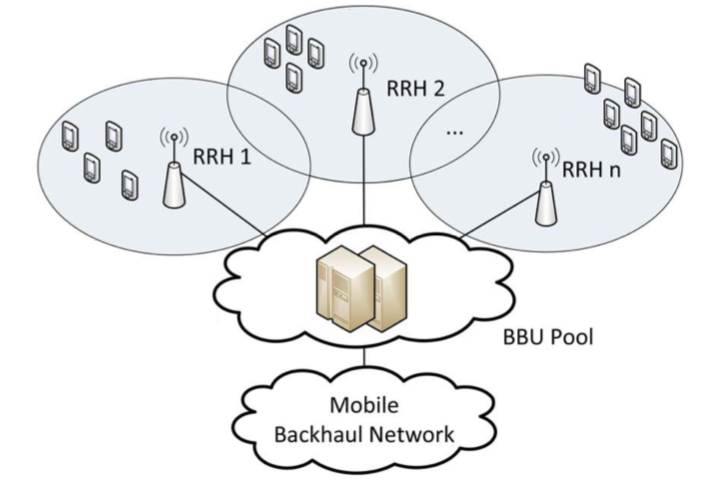
\includegraphics[width=0.6\textwidth]{images/cran}
	\caption{C-RAN}
	\label{fig:cran}
\end{figure}

\subsection{Objectives and performance indexes}
The objective of the study is to determine if and under which conditions it is better to perform packet compression or not.
For a correct evaluation of the system will be taken as reference the mean end-to-end delay of packets.

\newpage

\section{Model}
The model based to the queueing theory is shown in Figure~\ref{fig:model}.
We have $ N + 1 $ service centers, one represents the BBU with its interarrival rate $ \lambda_{bbu} $, which corresponds to the external arrival rate $ \gamma $ of the whole system, and service rate $ \mu_{bbu} $, the other N ones represent the RRHs with their $ \lambda_{rrh} $ and $ \mu_{rrh} $. Packets that leave the BBU have the same probability to reach the i-th RRH (i.e. $ \pi_{i} = \pi \text{ } \forall i $).
\begin{figure}[h]
	\centering
	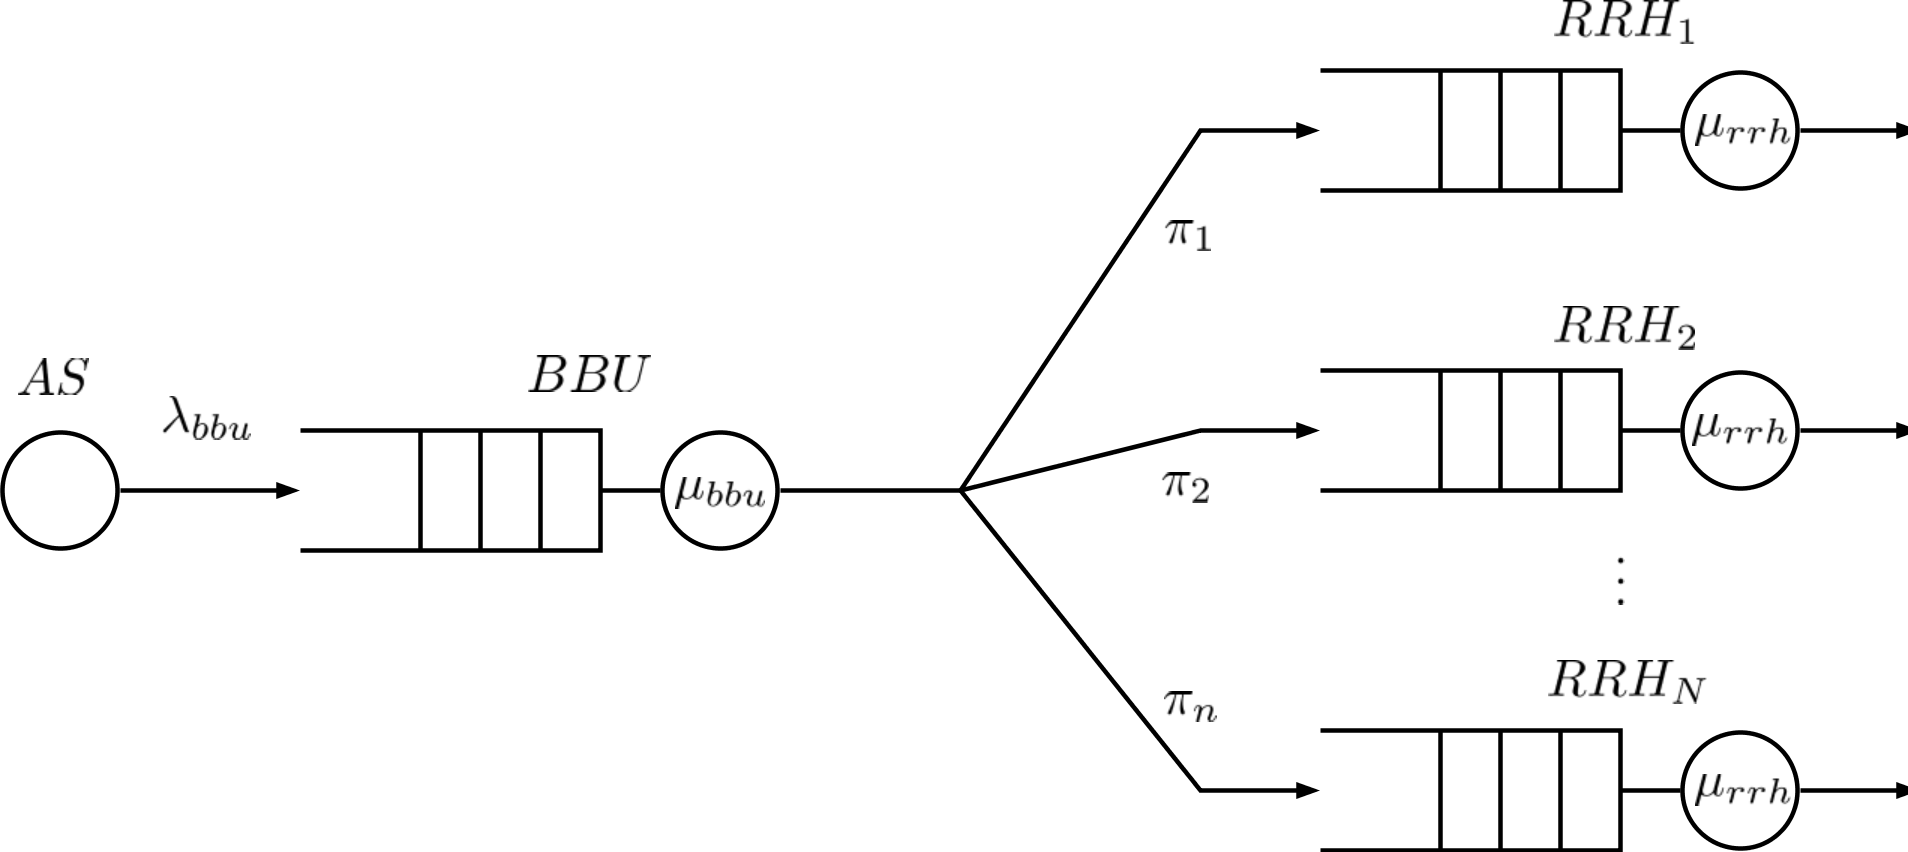
\includegraphics[width=0.6\textwidth]{images/model}
	\caption{Queueing network model}
	\label{fig:model}
\end{figure}

We make some semplifications which do not affect the final results:
\begin{itemize}
    \item time to reach the next service center is negligible;
    \item BBU switching time (time needed to change the output gate) is negligible;
    \item compression time on BBU is negligible;
    \item packets are not corrupted;
    \item no packet loss at the buffers (infinite buffers).
\end{itemize}

With these assumptions, we can compute the end-to-end delay in the following way:

% METTERE I MEAN?

$$ T_{delay} =  T_{waiting\_bbu} + T_{transmission} + T_{waiting\_rrh} + T_{decompression} $$

where 

$$ T_{transmission} = \frac{1}{\mu_{bbu}} = \frac{s}{X} $$

and

$$ T_{decompression} = \frac{1}{\mu_{rrh}} = C \cdot 50ms $$

\subsection{Validation}
The simulator has been validated through a comparison with a queueing theory model of the system.

The system has been modelled as an Open Jackson Network because all the hypotheses are verified since external arrivals are poissonian and routing probabilities are state-independent because they are uniform as specified in the requirements.

\subsubsection{Stability conditions}
In order to compute the stabilty conditions we have to distinguish between the two cases. In all equations we use the mean value of parameters and factors.

In case A we have to respect only one condition regarding the BBU. Indeed, on the RRHs we will never have queues because when the packet arrives it is immediately consumed.
Hence, the stability condition for the whole system, without compression, is the following:

$$ \lambda_{bbu} < \mu_{bbu}, \quad \lambda_{bbu} = \frac{1}{t}, \quad \mu_{bbu} = \frac{X}{s}$$

\begin{equation} \label{eq:rho-bbu}
\rho_{bbu} = \frac{\lambda_{bbu}}{\mu_{bbu}} = \frac{s}{t \cdot X} < 1
\end{equation}

Note that $s$ represents the number of bytes that the BBU has to transmit:
$$s = s_{original}\cdot(1-\frac{C}{100})$$

In case B we have also to take in account the stability condition on the RRHs because, in a system that foresees compression, the RRH service time is not null and depends on the compression percentage. 

Moreover, we have to consider the arrival rate on RRHs.
We have to guarantee that the latter is poissonian. If we consider just one RRH, the model can be seen as a tandem QN which respects Burke's theorem, since queues are infinte by our semplifications. Hence, the arrival rate at the RRH is a Poisson process with rate $ \lambda_{bbu} $ regardless of the BBU service rate, that, in our simulations, will be both exponential and lognormal. 
In a system with more than one RRH, any probabilistic splitting of a Poissonian process still originates Poissonian processes. Each RRH arrival rate will depend on the $ \lambda_{bbu} $ and on the number of remote radios as follows:

$$ \lambda_{rrh} = \lambda_{bbu} \cdot \pi = \frac{1}{t \cdot N} $$

$$ \mu_{rrh} = \frac{1}{C \cdot k}, \quad k = 50ms $$

\begin{equation} \label{eq:rho-rrh}
\rho_{rrh} = \frac{\lambda_{rrh}}{\mu_{rrh}} = \frac{C \cdot k}{t \cdot N} < 1
\end{equation}

Hence, using the result obtained in \ref{eq:rho-bbu}, the final stability condition for case B is:

$$ \begin{cases} \rho_{bbu} = \frac{s}{t \cdot X} < 1 \\ \\ \rho_{rrh} = \frac{C \cdot k}{t \cdot N} < 1 \end{cases} $$

with steady state probability, either on BBU and RRHs, equal to:

$$ p_{n} = \rho^n \cdot (1 - \rho) $$

Note that the steady state probability on each RRH and on the BBU is equal to an M/M/1.

\subsection{Statistics for validation}
In order to validate our model we have used the following perfomance indexes taken from the queueing theory:

$$ E[N_{bbu}] = \frac{\rho_{bbu}}{1 - \rho_{bbu}} = \frac{s}{X \cdot t - s} \text{, } E[R_{bbu}] = \frac{E[N_{bbu}]}{\lambda_{bbu}} =  \frac{s \cdot t}{X \cdot t - s}$$

$$ E[N_{rrh}] = \frac{\rho_{rrh}}{1 - \rho_{rrh}} = \frac{C \cdot k}{t \cdot N - C \cdot k} \text{, } E[R_{rrh}] = \frac{E[N_{rrh}]}{\lambda_{rrh}} = \frac{C \cdot k \cdot t \cdot N}{t \cdot N - C \cdot k}$$
\\

The successful comparison between these equations and the simulator results assure us that we are working on a correct model for our system.

\section{Simulator implementation}
The simulator consists of four modules as shown in Figure~\ref{fig:simulator}:
\begin{itemize}
  \item \texttt{As}: it creates/produces a packet flow according to the interarrival time sending them to the BBU;
  \item \texttt{Bbu}: it forwards the packets received from the AS to the RRH, compressed if it has to;
  \item \texttt{Rrh}: it decompresses the packet, if it was compressed, and sends it to the collector for the delay statistics;
  \item \texttt{Collector}: it handles of the delay statistics.
\end{itemize}

\begin{figure}[h]
    \centering
    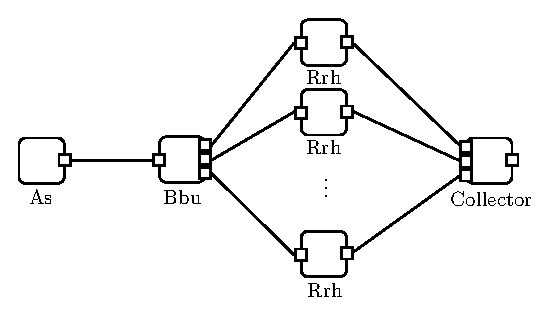
\includegraphics[width=0.6\textwidth]{images/simulator}
    \caption{Simulator architecture}
    \label{fig:simulator}
\end{figure}

\subsection{Application Server (AS)}
The As module has to perform cyclically the following operations:
\begin{itemize}
    \item[1.] it creates a new packet with the \texttt{id}, the packet size \texttt{s} taken either from an exponential distribution or a lognormal one, the destination taken from an uniform distribution, the creation time \texttt{created\_at};
    \item[2.] it sends the packet to the BBU;
    \item[3.] it waits according to the interarrival time \texttt{t} taken from an exponential distribution.
\end{itemize}

\subsection{Baseband Unit (BBU)}
When the Bbu module receives a packet from the AS it has to do the following actions:
\begin{itemize}
    \item[1.] if it is idle, it processes the packet immediately, otherwise the packet will be queued and served using a FIFO policy;
    \item[2.] it processes the packet deciding whether the packet must be compressed or not and transmitting it to the proper RRH;
    \item[3.] if there are any other packets in the queue, the first of them is pulled off from the buffer and served, otherwise it waits for the next packet.
\end{itemize}

\subsection{Remote radio (RRH)}
When one of the N RRHs receives a packet from the BBU, it acts as follow:
\begin{itemize}
    \item[1.] if it is idle, it processes the packet immediately, otherwise the packet will be queued and served using a FIFO policy;
    \item[2.] it processes the packet deciding whether the packet must be decompressed or not and transmitting it to the Collector;
    \item[3.] if there are any other packets in the queue, the first of them is pulled off from the buffer and served, otherwise it waits for the next packet.
\end{itemize}


\subsection{Collector}
The Collector module (virtually) collects all the packets coming from the RRHs and deals with the end-to-end delay statistics.

\section{Verification}
The simulator has been verified in order to check for memory leaks and bugs.
For the first ones we have used Valgrind tool, whereas, for bugs, we have done some simulations with known results.

We have set proper values, for both \texttt{warmup-time} and \texttt{simulation-time-limit}, according to some simulation results.
\begin{figure}[h]
	\centering
	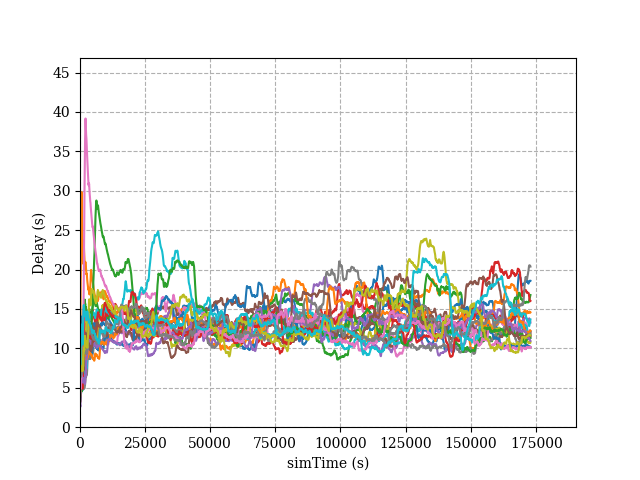
\includegraphics[width=0.6\textwidth]{images/warm-up}
	\caption{Warm-up study}
	\label{fig:warm-up-study}
\end{figure}

We have estimated the \texttt{warmup-time} applying the sliding window average (windowSize = 10000) to the mean end-to-end delay values obtained from 20 independent repetitions of our highest value of $ \rho_{bbu} $ (0.9). The same reasoning will be applied to the next simulations.

In Figure~\ref{fig:warm-up-study} it is shown that a good value for \texttt{warmup-time} is around 50000 seconds, where the initial transient is over and the steady state is reached. 

The value for the \texttt{simulation-time-limit} has been chosen in order to have enough results for statistics (i.e. 2 days of simulation time).

\section{Experiments}
We will analyze separately the two cases described in Section~\ref{sec:introduction} either with exponential and lognormal distribution, the latter only for the packet size.
We will take in account scenarios with at least 2 remote radios, because a system with only one remote radio is not interesting to analyze. Futhermore, the number of RRH has to verify the stability condition computed in \ref{eq:rho-rrh}. For each case we have done 20 different repetitions for every single scenario.

\subsection{Case A - Transmission without compression}
In this case the end-to-end delay could depend on two factors:
\begin{itemize}
	\item \texttt{X}, chosen such as $ \rho_{bbu} $, computed as in \ref{eq:rho-bbu}, will assume values from 0.1 to 0.9 increased by 0.1;
	\item \texttt{N}, with prefixed values of 2, 5, 10.
\end{itemize}
\subsubsection{Exponential}
Since the exponential distribution does not provide a variance control, the packet size \texttt{s}, extracted by the AS, could assume both small and large values.

In Figure~\ref{fig:case-a-exp}, as we expected, we can see that the end-to-end delay does not depend on the number of remote radios \texttt{N} because on the RRH the service time is null, so there will be no queues and the packets will be forwarded to the cells immediately.

In fact, the three different plots (2, 5 and 10 RRHs) overlap perfectly.
Hence, the end-to-end delay corresponds only to the BBU response time, so the only factor that allows us to minimize the end-to-end delay is the BBU transmission speed \texttt{X}.


%\begin{align}
%E[R] &= E[R_{bbu}] \notag \\
%&= E[W_{bbu}] + \frac{1}{\mu_{bbu}} \notag \\
%\end{align}
\subsubsection{Lognormal}
In the lognormal scenario, the probability to have packet size values greater than the mean value is higher with respect to the exponential distribution. For this reason the end-to-end delay (shown in Figure~\ref{fig:case-a-log}) tends to be higher than the previous analysis as \texttt{X} decreases.

Furthermore, we can notice that the confidence interval for lower values of \texttt{X} ($\rho \simeq 1$) is wider than the exponential one. This is due to the fact that the system is sensitive to an unlucky stream of packet whose size is greater than the mean size value.


\begin{figure}
\centering
\begin{subfigure}{.5\textwidth}
  \centering
  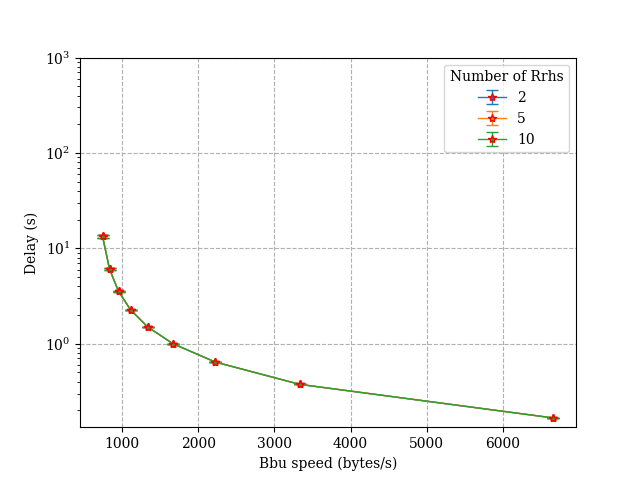
\includegraphics[width=\linewidth]{images/case-a-exp}
  \caption{Exponential distribution}
  \label{fig:case-a-exp}
\end{subfigure}%
\begin{subfigure}{.5\textwidth}
  \centering
  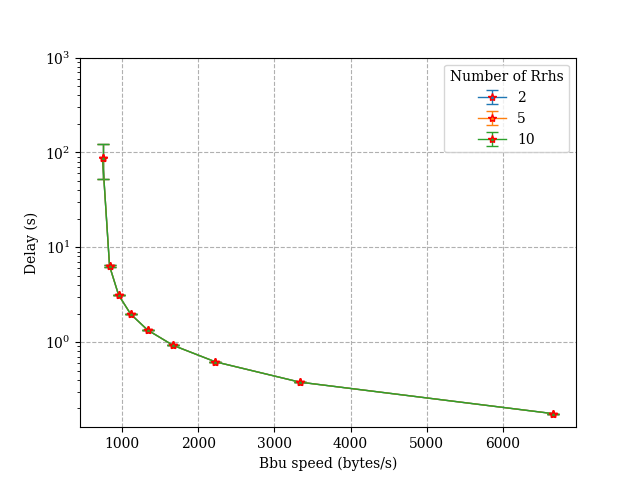
\includegraphics[width=\linewidth]{images/case-a-logn}
  \caption{Lognormal distribution}
  \label{fig:case-a-log}
\end{subfigure}
\caption{Case without compression}
\label{fig:case-a}
\end{figure}

Of course, also in this case, the only meaningful scalable factor is the BBU transmission speed.
\bigbreak
\noindent The data for both distributions have been tested with a level of confidence interval of 99\%. 

\subsection{Case B - Transmission with compression}
In addition to the factors of case A, now we have a further factor to take in account: the compression percentage. Hence, the set of factors becomes:

\begin{itemize}
	\item \texttt{X}, that will assume the same values of case A, but we have to consider that now $ \rho_{bbu} $ depends on the compression percentage because of the smaller number of bytes transmitted. We have chosen these values for the sake of a correct comparison between the two cases.
	\item \texttt{N}, with values ranging from 2 to 50.
	\item \texttt{C}, with values ranging from 10 to 90.
\end{itemize}

\subsubsection{Exponential}
According to inequality expressed in \ref{eq:rho-rrh}, $ \rho_{rrh} $ does not depend on \texttt{X}, thus, we can fix the BBU speed (i.e. 1000 bytes/s) and compare the waiting times obtained from the variations of \texttt{N} and \texttt{C}. In Figure~\ref{fig:c-vs-waiting-1} we can see the waiting time trend for compression values up to 90\% keeping in mind that we need at least 4 RRHs in order to satisfy the stability condition.

\begin{figure}
\centering
\begin{subfigure}{.5\textwidth}
  \centering
  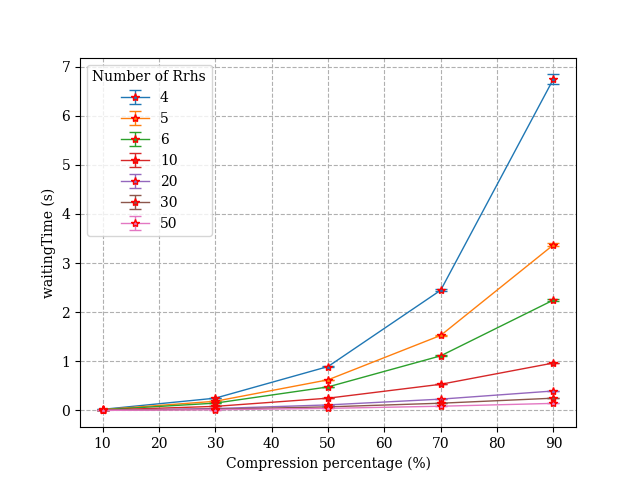
\includegraphics[width=\linewidth]{images/c-vs-waiting}
  \caption{Waiting time in relation to \texttt{C} and \texttt{N}}
  \label{fig:c-vs-waiting-1}
\end{subfigure}%
\begin{subfigure}{.5\textwidth}
  \centering
  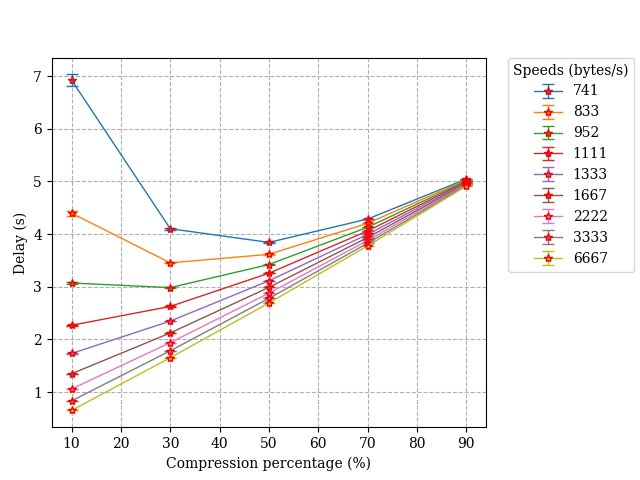
\includegraphics[width=\linewidth]{images/c-vs-delay}
  \caption{Delay with 20 RRHs}
  \label{fig:c-vs-delay}
\end{subfigure}
\caption{}
\label{fig:waiting-and-delay}
\end{figure}

As the number of RRHs increases, the waiting time tends to be constant around zero becoming independent from the compression percentage.

Hence, for this consideration, we can fix the number of RRH to an high value (i.e. 20) in order to have a negligible waiting time on the RRHs, and see how the end-to-end delay varies as BBU speed and compression percentage change (Figure~\ref{fig:c-vs-delay}).

\begin{figure}[b]
\centering
\begin{subfigure}{.5\textwidth}
  \centering
  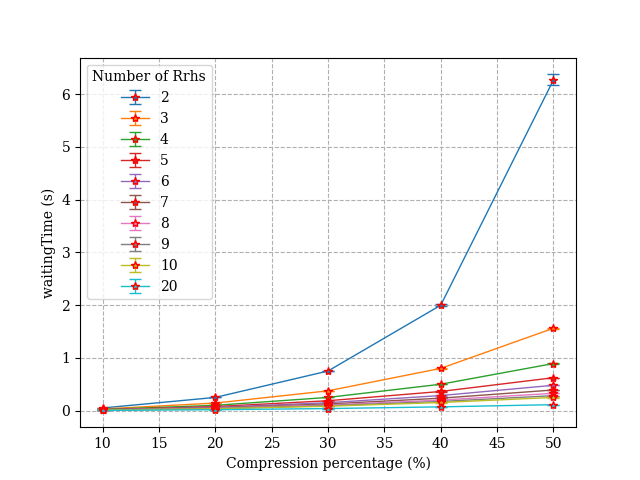
\includegraphics[width=\linewidth]{images/c-vs-waiting-from-2}
  \caption{Waiting time in relation to \texttt{C} and \texttt{N}}
  \label{fig:c-vs-waiting-2}
\end{subfigure}%
\begin{subfigure}{.5\textwidth}
  \centering
  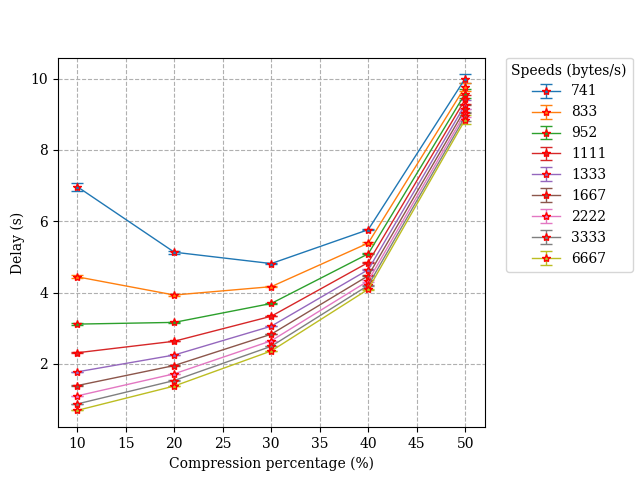
\includegraphics[width=\linewidth]{images/worst-case}
  \caption{Delay with 2 RRHs}
  \label{fig:worst-case}
\end{subfigure}
\caption{}
\label{fig:waiting-and-delay-2}
\end{figure}

As the speed increases (i.e. from 1111 bytes/s), the end-to-end delay tends to become a monotonically increasing function and it is not convenient to use higher compressions. Furthermore, also in this experiment where the waiting time on the RRH is negligible, for none of the BBU speeds taken into consideration there are not any advantages in setting the compression percentage over 50\%. For this reason, from now on, we will consider the compression percentage with values ranging from 10\% to 50\% allowing us to reach the stability condition even for 2 and 3 RRHs (Figure~\ref{fig:c-vs-waiting-2}).

Now we want to analyze the system with 2 RRHs, when we have the highest RRH waiting time, to see whether, with low BBU speeds, we still have advantages in increasing the compression percentage (Figure~\ref{fig:worst-case}).

We can observe that, in this case, for BBU speed equal to 952 bytes/s we do not have advantages in increasing \texttt{C} unlike the case shown in Figure~\ref{fig:c-vs-delay}. Instead, we still have advantages for both BBU speed values of 833 bytes/s and 741 bytes/s, the latter will be taken as example of our next study, where we are interested in seeing which is the best compression value for each meaningful \texttt{N}.

\begin{figure}[h]
\centering
  \centering
  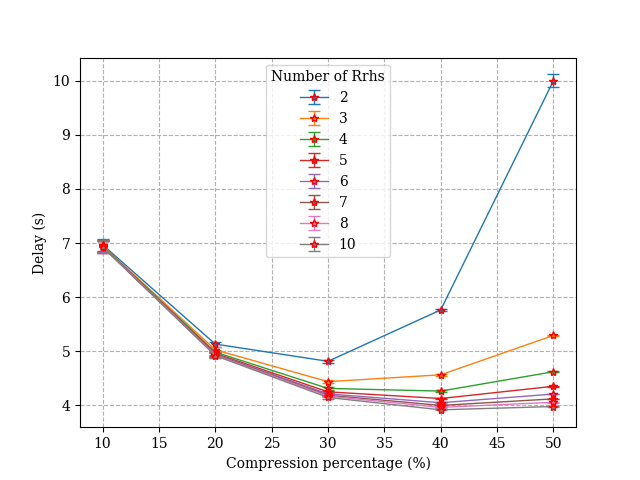
\includegraphics[width=0.5\textwidth]{images/c-vs-delay-741}
  \caption{Delay in relation to \texttt{C} and \texttt{N}, with \texttt{X}=741bytes/s}
  \label{fig:c-vs-delay-741}
\end{figure}


Figure~\ref{fig:c-vs-delay-741} shows that the value of \texttt{C}, that minimize the end-to-end delay, increases as \texttt{N} goes up. This is due to the fact that the workload is evenly distributed among the increasing number of remote radios. In Figure~\ref{fig:response-time} it is clearly shown how the delay is subdivided between BBU and remote radios.

\begin{figure}[h]
\centering
\begin{subfigure}{.5\textwidth}
  \centering
  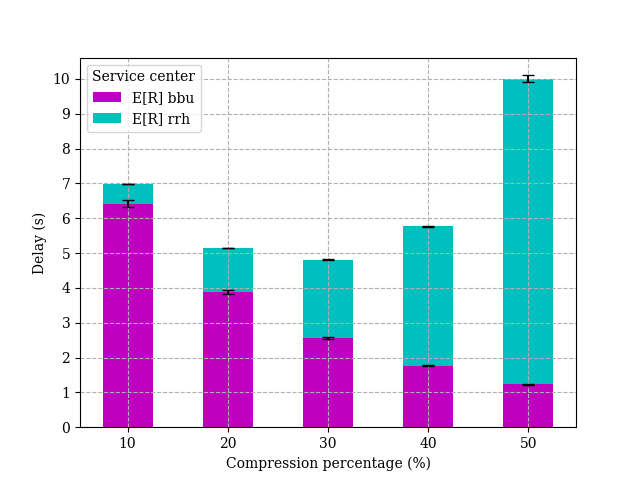
\includegraphics[width=\linewidth]{images/response-time-2}
  \caption{2 RRHs}
  \label{fig:response-time-2}
\end{subfigure}%
\begin{subfigure}{.5\textwidth}
  \centering
  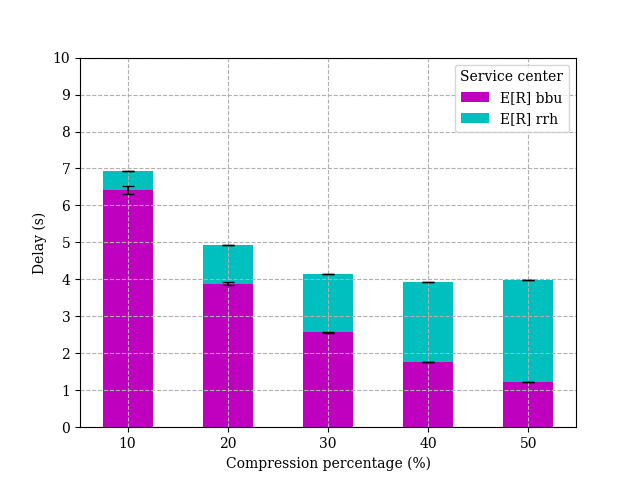
\includegraphics[width=\linewidth]{images/response-time-10}
  \caption{10 RRHs}
  \label{fig:response-time-10}
\end{subfigure}
\caption{End-to-end delay ratio}
\label{fig:response-time}
\end{figure}

\newpage

\subsubsection{Lognormal}
As we have seen in case A, for $\rho \simeq 1$ (in our case \texttt{X}=741bytes/s), the end-to-end delay, which is affected only by the BBU response time, assumed very high values and suffered a large variance. In case B we will not have anymore this situation due to the fact that the BBU transmits less bytes depending on \texttt{C}. Considering that $\rho_{bbu}$ is computed as in \ref{eq:rho-bbu} and \texttt{s} is reduced by \texttt{C}, its value (for equal \texttt{X} of case A) will be lower and consequently the BBU will stabilize first (Figure~\ref{fig:c-vs-resp-741-logn}).

\begin{figure}[h]
	\centering
	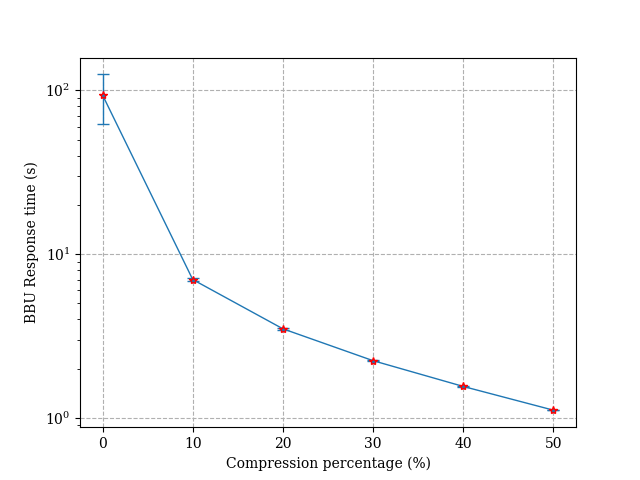
\includegraphics[width=0.5\textwidth]{images/response-time-bbu-741-logn}
	\caption{BBU response time lognormal distribution in relation to \texttt{C}, with \texttt{X}=741bytes/s}
	\label{fig:c-vs-resp-741-logn}
\end{figure}

By Burke's theorem the lognormal distribution will affect only the BBU statistics, that are similar to the exponential ones (Figure~\ref{fig:c-vs-response-time-bbu}). As the RRHs behavior will not be affected by a different distribution, the two configurations of the system gave similar trends. 

When $\rho_{bbu}$ goes up the performance of the lognormal distribution is worse than the exponential one, instead for lower values of $\rho_{bbu}$ we have a slightly increased performance. However, due to the trends redundancy, for the lognormal distribution we can refer to the exponential study.

\begin{figure}[h]
	\centering
	\begin{subfigure}{.5\textwidth}
		\centering
		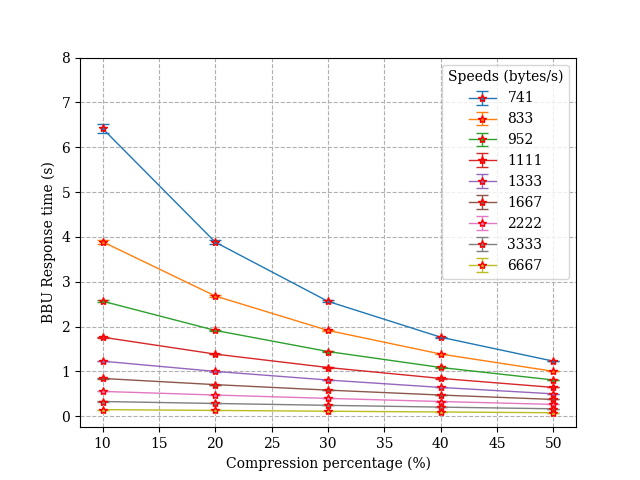
\includegraphics[width=\linewidth]{images/c-vs-response-time-bbu-exp}
		\caption{Exponential distribution}
		\label{fig:c-vs-response-time-bbu-exp}
	\end{subfigure}%
	\begin{subfigure}{.5\textwidth}
		\centering
		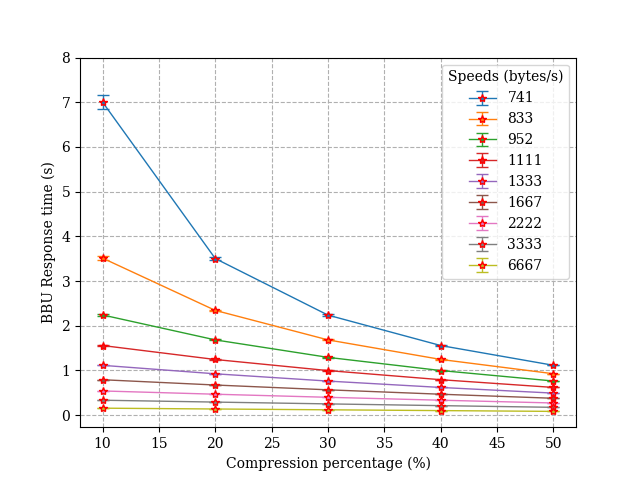
\includegraphics[width=\linewidth]{images/c-vs-response-time-bbu-logn}
		\caption{Lognormal distribution}
		\label{fig:c-vs-response-time-bbu-logn}
	\end{subfigure}
	\caption{BBU response time in relation to \texttt{C} and \texttt{X}}
	\label{fig:c-vs-response-time-bbu}
\end{figure}

\subsection{Comparison}

The main objective of this study is to establish when and with which compression percentage we can have lower values of the end-to-end delay. As we have seen, for \texttt{C} equal to 0, \texttt{N} is irrelevant for the puposes of the end-to-end delay study, and in Figure~\ref{fig:c-vs-delay-741} is shown that for \texttt{N} greater than 5 the delay behaviors tends to comply. Hence for the comparison study we fix \texttt{N} equal to 5. 

\begin{figure}[h]
	\centering
	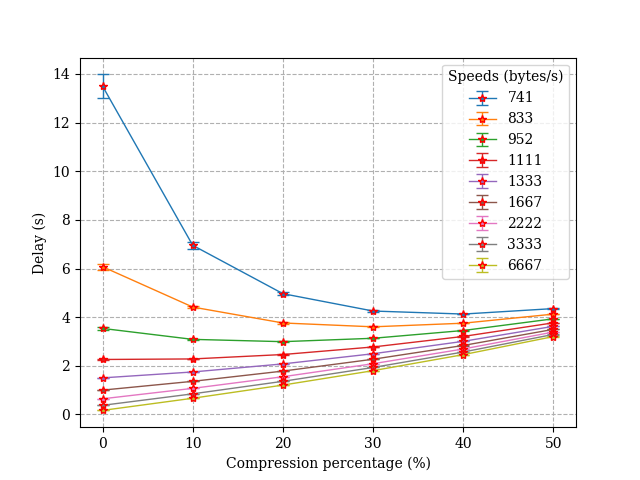
\includegraphics[width=0.5\textwidth]{images/c-vs-delay-comparison}
	\caption{Delay in relation to \texttt{C}, \texttt{N} = 5} 
	\label{fig:c-vs-delay-comparison}
\end{figure}

For a certain \texttt{X} value onward, in our case 1111 bytes/s, we will not have any benefits in using this compression algorithm because the time saved in transmitting lower number of bytes is not rewarded by the longer time spent on the RRH.
On the other hand, below this \texttt{X} value, the compression increases the performance. 

From Figure~\ref{fig:c-vs-delay-comparison} we can only estimate an interval of \texttt{C} where we obtain the lower delay for a given \texttt{X}; for the exponential distribution we could obtain a more accurate value studying the following inequality, remembering that the RRH response time is null when there is no compression:

\begin{equation} \label{eq:inequality}
E[R_{bbu}]_{comp} + E[R_{rrh}] < E[R_{bbu}]
\end{equation}
\\
Considering \texttt{C} as variable and fixing \texttt{N} and \texttt{X}, we obtain a parabolic function whose vertex gives us the optimal compression percentage.

For example, with \texttt{X} = 741 bytes/s, from the graph we can estimate the best value of \texttt{C} between 30\% and 50\%. The computation of \ref{eq:inequality} confirms our estimation giving 48\% as result.

\newpage
\section{Conclusions}
This project analyzed a CRAN system which can adopt a compression/decompression algorithm whose compression time is null and decompression time depends on the percentage adopted.\\
Thus we studied the trend of the mean end-to-end delay in relation to \texttt{C}: 
\begin{itemize}
	\item For lower values of \texttt{C} it is more convenient increasing \texttt{X} instead of \texttt{N}. Indeed, for $\texttt{C} = 0 $ the number of remote radios is irrelevant.
	\item For high values of \texttt{C} it is more convenient increasing \texttt{N} instead of \texttt{X}. This is true for \texttt{N} up to 20, after that increasing the number of remote radios brings meaningless improvements.
\end{itemize}
For the range of analyzed values, the benefits brought by compression can be appreciated only at lower BBU transmission speeds where the time gained by size reduction is greater than the time spent on the RRH because of decompression. Increasing the number of RRH, thus decreasing the workload on them, the value of \texttt{C}, that gives the shortest end-to-end delay, increases.



\end{document}